%source mathadata
\begin{multicols}{2}
		Pour séparer les nuages de points, on propose la droite passant par les points $A(1;2)$ et $B(3;3)$.
		\begin{MADenumerate}
			\item Calculer le coefficient directeur de la droite, à partir des coordonnées de $A$ et $B$.
			\item Déterminer $p$ en remplaçant $x$ et $y$ par les coordonnées de $A$ dans l'équation $y=mx+p$. (N'oubliez pas de remplacer $m$ aussi.)
			\item Donner l'équation de la droite.
			\item Tracer la droite $(AB)$. Par lecture graphique, les valeurs de $p$ et de $m$ vous semblent-elles correctes ?
		\end{MADenumerate}

		%\columnbreak

		\begin{center}
			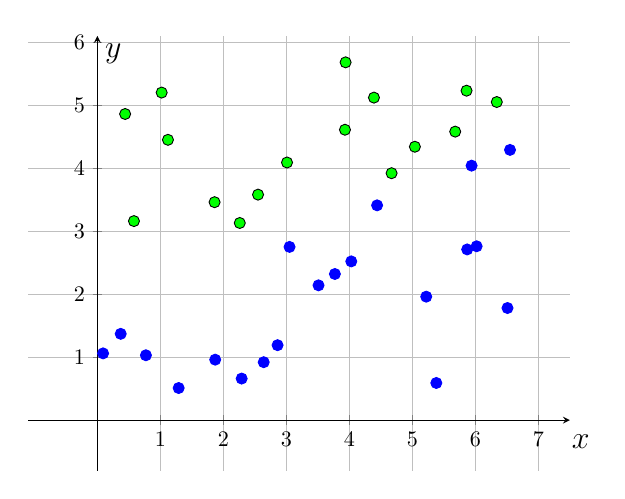
\begin{tikzpicture}[scale=0.8]
				\begin{axis}[
						x=1cm,y=1cm,
						axis lines=middle,
						ymajorgrids=true,
						xmajorgrids=true,
						xmin=-1.1,
						xmax=7.5,
						ymin=-0.8,
						ymax=6.1,
						xtick={1,...,7},
						ytick={0,1,...,6},
						xlabel={\Large $x$},
						xlabel style={at={(axis description cs:1.02,0.1)}, anchor=north},
						ylabel={\Large $y$},
						clip=true
					]
					\clip(-0.2,-0.2) rectangle (8,6);

					% Classe A (points bleus) -- majoritairement en dessous de y = 0.5 x + 1.5
					\addplot[only marks,mark=*,mark size=2.5pt,draw=blue, fill=blue] coordinates {
							(0.37,1.37) (1.87,0.96) (3.05,2.75) (2.64,0.92)
							(6.55,4.29) (0.77,1.03) (5.87,2.71) (1.29,0.51)
							(5.94,4.04) (4.44,3.41) (2.86,1.19) (6.02,2.76)
							(5.22,1.96) (3.51,2.14) (3.77,2.32) (2.29,0.66)
							(6.51,1.78) (0.09,1.06) (4.03,2.52) (5.38,0.59)
						};

					% Classe B (points noirs) -- majoritairement au-dessus de y = 0.5 x + 1.5
					\addplot[only marks,mark=*,mark size=2.5pt,draw=black, fill=green] coordinates {
							(3.94,5.68) (1.12,4.45) (3.01,4.09) (5.86,5.23)
							(1.86,3.46) (0.44,4.86) (2.26,3.13) (3.93,4.61)
							(4.39,5.12) (1.02,5.20) (5.04,4.34) (0.58,3.16)
							(2.55,3.58) (4.67,3.92) (5.68,4.58) (6.34,5.05)
						};

					% Séparatrice (p = 1.5, pente 0.5)
					% \addplot[domain=-0.5:7, samples=2, thick] {0.5*x + 1.5};
				\end{axis}
			\end{tikzpicture}
		\end{center}

	\end{multicols}
